%!TEX root = ../crimson_throne_book_main.tex
% 2015-01-17
Looking at the cadaver of the brown bear that the ogrekin's hunting dogs took down, Balian realizes it has a nice, thick pelt that would make an excellent rug for his bedroom. With Puk's aid he starts skinning the magnificent animal, while Sjo tries his hand at preparing a juicy bear steak. When the companions finally return to the road where they left their horses, they are surprised to find their mounts missing. Fortunately whoever took them did not bother about hiding his tracks, so Balian easily picks up a trail. About an hour down the road the heroes discover two wooden buildings off the road, next to a clearing in the wood.\\

Puk sneaks closer to scout ahead. The two sagging buildings look like a worn down hunting lodge and barn. Windows have been boarded over and moss and fungus grow on the shaded sides of the decrepit structures. The halfling also spots a tangled field of corn and other diseased plants growing in the clearing.\hyperref[fig:Crowfood-Graul-507695369]{ An eight-foot tall brute } is working the ground with a vicious iron hook. His grotesquely deformed head resembles a giant pumpkin: a huge mass of tumors and overgrown bone gives his head a lopsided look. Numerous crows fill the air above him. Puk circles the lodge, sticking to the trees, and makes his way around the building to the barn. Upon approaching that building he quickly makes out the frightened whinnying of horses, cruel chuckles of more brutes and savage snarls of dogs inside. \\

\begin{figure}[h]
	\centering
	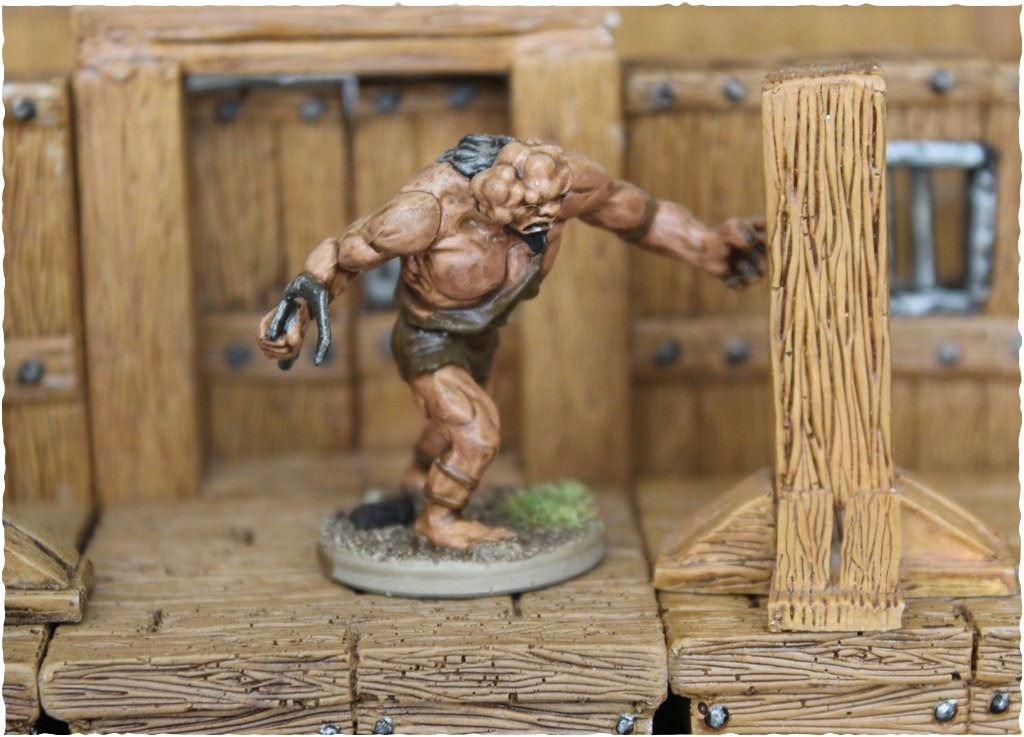
\includegraphics[width=0.4\textwidth]{images/Crowfood-Graul-507695369_mod.jpg}
	\caption{Crowfood Graul}
	\label{fig:Crowfood-Graul-507695369}
\end{figure}

The halfling gathers his friends and together they stealthily crawl up to front of the barn. Puk throws open the doors and the companions look upon an unpleasant scene.\hyperref[fig:Graul-barn-507694269]{ Three ogrekin } and two skinny, naked dogs are torturing three awkwardly bound horses. Puk's riding animal seems to be taking the worst punishment and shows various cut and bite marks. Balian's and Sjo's mount are here as well, but there is no immediate sign of Quint's ride. Balian storms in, charging an ugly ogrekin who has two forearms growing from his right elbow. Quint swirls his whip around the crooked stumpy legs of an exceptionally short hillbilly and pulls him to the ground, so Puk can stab him in a weak spot while he's down. Meanwhile Sjo realizes that the third of the brothers in the barn is huge, even in his eyes, standing over eight and a half feet tall. This giant has a somewhat 'normal' face, although his eyes are very big and his skin is pale as the full moon. Balian wields his weapon to great efficiency, taking out one of the dogs and the short-legged brother in one mighty sweep. He next faces the wrath of the two remaining brothers, who hit him hard with their bare hands. Meanwhile the pumpkin-headed ogrekin who was working the field outside, has rushed to his brothers' aid. He throws himself on Sjo, dangerously whirling around his vicious iron hook. Balian and Puk take out another opponent: the tall hulk falls dead at their feet. The last of the three torturers smashes the ranger in return with his twin forearms, but Quint understand that fourth, pumpkin-headed brother is the biggest threat, as he is clearly more experienced in battles and packs a ferocious punch. The bard spellbinds the ugly brute with a successful  {\itshape cacophonous call} , causing a sickening head-ache to surge through his tumorous brain, taking away his ability to fight. The creature retreats to the door and flees the scene. In the meantime the companions finish off the last opposition in the barn, before chasing after the ogrekin who is fleeing around the barn. The heroes manage to corner him and - even though he regains control of his actions and dishes out some damage to Spyder - he succumbs quickly to superior numbers. \\

\begin{figure}[h]
	\centering
	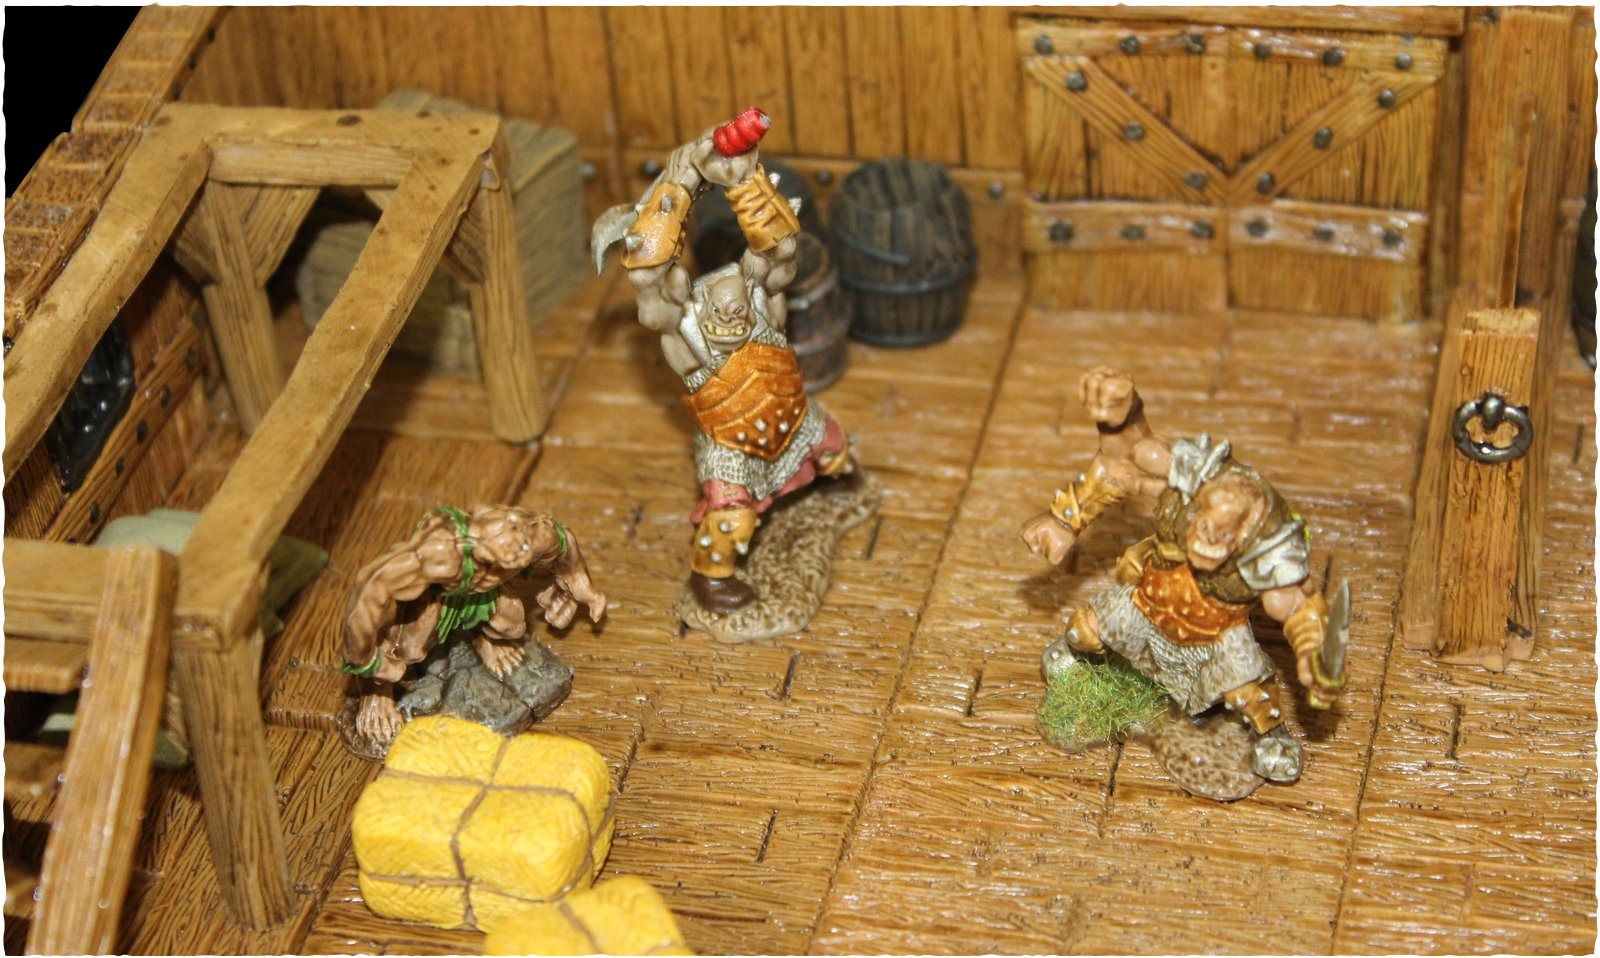
\includegraphics[width=0.4\textwidth]{images/Graul-barn-507694269_mod.jpg}
	\caption{Graul barn}
	\label{fig:Graul-barn-507694269}
\end{figure}

With Quint's horse still missing, the companions decide to tackle the main house next. This decaying hunting lodge slumps drunkenly at the edge of the clearing. Rickety stairs crawl up to a porch covered by a huge eave which is supported by heavy pillars of pine. These timbers have crude carvings of manticores impaling children and wolves ripping apart women. The simple decorations look like a child's work, but the depictions grow more gruesome from one picture to the next. A large rocking chair of lashed wood and bone sways erratically in the breeze at the far end of the porch under a vast menagerie of wind chimes, all composed of humanoid and animal bones. The windows have been boarded up with thick timbers, although it is unclear whether this is to keep intruders out or to keep unspeakable horrors in. A host of ants marches happily away, many the size of a grown man's thumbnail. A moth as big as a shovel-head clings to the porch ceiling, watching the party with alienating eyes. The scent of bad meat, urine, sweat and decay wafts from between the cracks.\\

Sjo's warning that there might be traps is merrily laughed away, but when Puk walks up to the front door, a rack mounted with a series of sharpened bones suddenly swings down from between the many hanging bones. At the same time rusty saw blades spring from the cracks in the floorboards. The terrible double trap fails to hurt the lucky halfling, though, as the spikes only pierce the air above Puk's head, while the blades slides just left and right from where he's standing, cutting off no more than a few hairs from the tufts covering his ever-bare feet. The halfling chuckles at his own good fortune and slowly pushes open the door. The reception room holds a tremendous hearth in the right wall, but there is no fire burning in it, while the small rogue remembers that smoke arose from the chimney on the roof. A mangy dire bearskin rug lies before the fireplace. The animal's pained visage still snarls at whatever hunter that took its life. To the left is a huge couch, haphazardly upholstered in animal hide and humanoid flesh. Sjo recognizes a fox's head and a human-looking hand and foot in the putrid leather collection. The door on the other side of the room has a big hole in the bottom, big enough for Puk to see that the hallway behind it is clear. After having crawled through the hole, the rogue's keen ears pick up the exhausted cracking of wood. It comes from the door to his left, causing his curiosity to rear its head.\\

The halfling leads his friends down the hall and quietly opens the door. Next Balian storms in and faces an incredibly corpulent woman with stringy, black hair, greasily sticking to her humongous head. She wears an old stained curtain as a robe.\hyperref[fig:Mammy-Graul-and-ogre-Daddy-507696824]{ The room } reeks of sweat, but also of decay, which originates from the chamber's second occupant, a hulking ogre who did not come into view until Balian charged inside. The ranger realizes that this giant is no longer alive, although he still moves to attack the intruders. Could this be the deformed ogrekin's mother in the company of their late father, returned from the dead? It certainly seems so. Disgusted by the foul woman the ranger chokes and fails to hit her. "I don't know who you are, strangers, but you are fools for coming in here! I'll have your heads on a pike to decorate my porch! Daddy, tear them apart!" she shrieks. Balian turns to the ogre zombie and decides to attack him first. His greatsword tears through the rotting meat while Puk tumbles through the room to find an advantageous flanking position behind the undead hulk. The zombie moans and swings his heavy greatclub at Balian, but the ranger can block his strike. The fat lady rolls around in her bed - obviously the source of the creaking Puk heard earlier - and throws a heinous spell at the halfling which  {\itshape blinds} him. With one simple incantation she has stolen the rogue most powerful weapon, his eye for weak spots. Quint recognizes the woman's threat and tries to take her out of the fight with a  {\itshape cacophonous call} , but she resists his magic through sheer power of will. Sjo bludgeons her with his heavy mace, but cannot prevent her from draining Balian's strength with a  {\itshape ray of enfeeblement} . The sly mage has now crippled the second damage dealer with her magic. Balian gets no time to recover, for the ogre crushes half his ribs with a devastating blow. Quint attempts another  {\itshape cacophonous call} on the fat lady, but her will proves too powerful again. Sjo rushes to Balian's aid with a healing spell so the ranger can continue the fight, but the undead ogre hits about wildly, wounding all the companions. With Puk's and Balian's efficiency greatly reduced, it is hard for our friends to bring the giant to his knees. Both Spyder and his master go down first, before Puk can finally deliver the finishing cut. Meanwhile Sjo has resorted to firing wave upon wave of  {\itshape burning hands} at the corpulent monster, who finds no protection from this magic among her five  {\itshape mirror images} . When her zombie bodyguard is beaten, she decides to play it safe and whispers the words of a powerful spell that  {\itshape dimension doors} her out of the room with a simple "poof". \\

\begin{figure}[h]
	\centering
	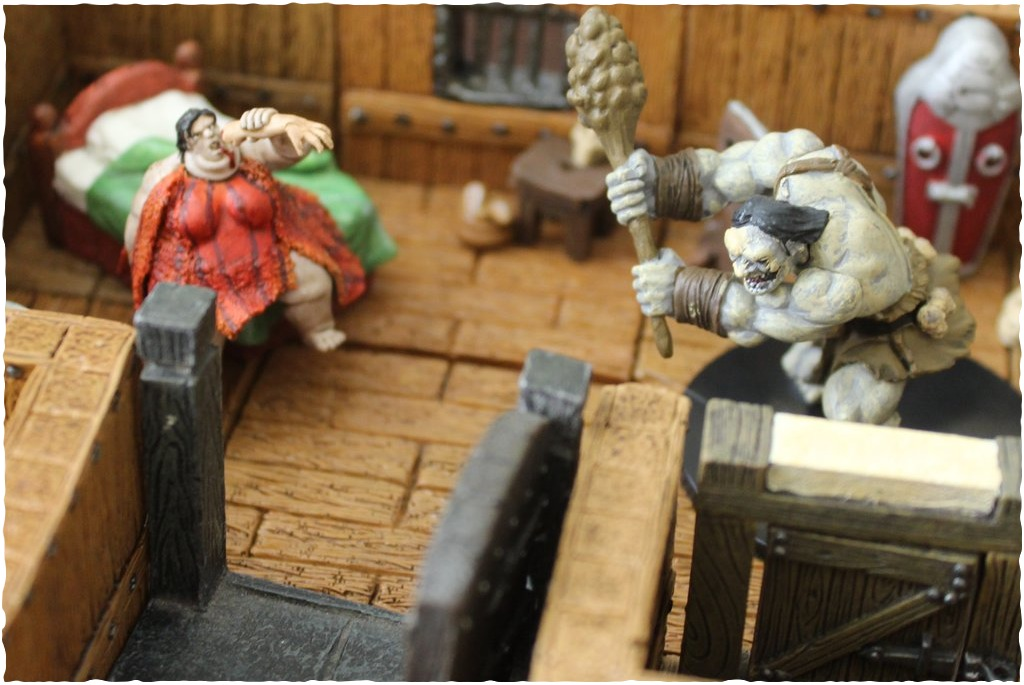
\includegraphics[width=0.4\textwidth]{images/Mammy-Graul-and-ogre-Daddy-507696824_mod.jpg}
	\caption{Mammy Graul and ogre Daddy}
	\label{fig:Mammy-Graul-and-ogre-Daddy-507696824}
\end{figure}

